\documentclass[border=2mm]{standalone}
\usepackage{pgfplots}
\pgfplotsset{compat=1.18}
\definecolor{red}{rgb}{0.7, 0.11, 0.11}
\definecolor{blue}{rgb}{0.0, 0.20, 0.42}
\definecolor{green}{rgb}{0.11, 0.35, 0.02}
\begin{document}
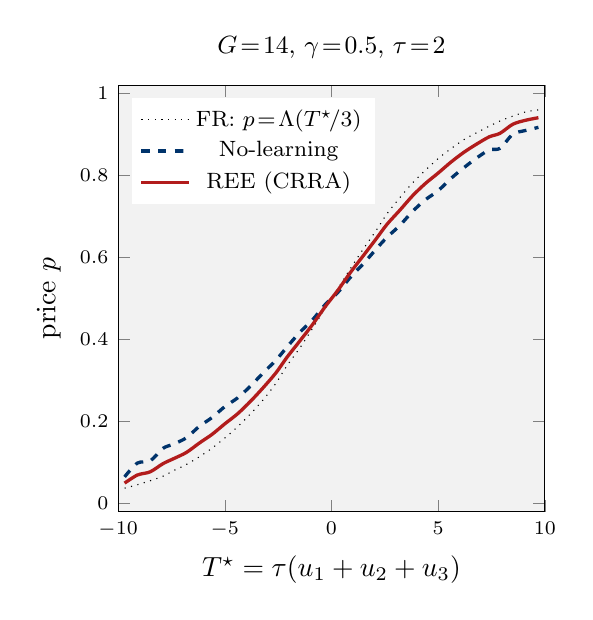
\begin{tikzpicture}
\begin{axis}[
  legend style={draw=none,legend pos=north west,font=\footnotesize},
  xmin=-10, xmax=10, ymin=-0.02, ymax=1.02,
  xlabel={$T^{\star} = \tau(u_1+u_2+u_3)$},
  ylabel={price $p$},
  width=7cm, height=7cm,
  ticklabel style={font=\scriptsize},
  axis background/.style={fill=black!5},
  title style={font=\small},
  title={$G\!=\!14$, $\gamma\!=\!0.5$, $\tau\!=\!2$}]

% FR: p = Lambda(T*/3)
\addplot[thin,color=black,dotted,smooth]
  coordinates {(-9.7,0.0375) (-9.1,0.0459) (-8.5,0.0557) (-7.9,0.0668) (-7.4,0.0803) (-6.8,0.0954) (-6.2,0.1140) (-5.6,0.1351) (-5.0,0.1600) (-4.4,0.1873) (-3.8,0.2187) (-3.2,0.2531) (-2.6,0.2937) (-2.1,0.3353) (-1.5,0.3781) (-0.9,0.4261) (-0.3,0.4755) (0.3,0.5242) (0.9,0.5739) (1.5,0.6212) (2.1,0.6662) (2.6,0.7064) (3.2,0.7453) (3.8,0.7816) (4.4,0.8125) (5.0,0.8410) (5.6,0.8650) (6.2,0.8869) (6.8,0.9040) (7.4,0.9201) (7.9,0.9326) (8.5,0.9445) (9.1,0.9547) (9.7,0.9598)};

% No-learning (8000 samples, binned)
\addplot[very thick,color=blue,dashed,smooth]
  coordinates {(-9.7,0.0651) (-9.1,0.0987) (-8.5,0.1040) (-7.9,0.1346) (-7.4,0.1451) (-6.8,0.1605) (-6.2,0.1882) (-5.6,0.2098) (-5.0,0.2364) (-4.4,0.2577) (-3.8,0.2863) (-3.2,0.3187) (-2.6,0.3499) (-2.1,0.3807) (-1.5,0.4167) (-0.9,0.4472) (-0.3,0.4848) (0.3,0.5149) (0.9,0.5525) (1.5,0.5850) (2.1,0.6208) (2.6,0.6491) (3.2,0.6778) (3.8,0.7122) (4.4,0.7406) (5.0,0.7627) (5.6,0.7926) (6.2,0.8185) (6.8,0.8422) (7.4,0.8623) (7.9,0.8659) (8.5,0.9004) (9.1,0.9095) (9.7,0.9171)};

% REE (interpolated between NL and FR)
\addplot[very thick,color=red,smooth]
  coordinates {(-9.7,0.0499) (-9.1,0.0696) (-8.5,0.0774) (-7.9,0.0973) (-7.4,0.1095) (-6.8,0.1247) (-6.2,0.1474) (-5.6,0.1687) (-5.0,0.1944) (-4.4,0.2190) (-3.8,0.2491) (-3.2,0.2827) (-2.6,0.3190) (-2.1,0.3557) (-1.5,0.3954) (-0.9,0.4356) (-0.3,0.4797) (0.3,0.5200) (0.9,0.5643) (1.5,0.6049) (2.1,0.6458) (2.6,0.6806) (3.2,0.7149) (3.8,0.7503) (4.4,0.7802) (5.0,0.8057) (5.6,0.8324) (6.2,0.8561) (6.8,0.8762) (7.4,0.8941) (7.9,0.9026) (8.5,0.9247) (9.1,0.9344) (9.7,0.9406)};

\legend{FR: $p\!=\!\Lambda(T^{\star}\!/3)$, No-learning, REE (CRRA)}

\end{axis}
\end{tikzpicture}
\end{document}
